\documentclass[12pt]{article}

\usepackage[english]{babel}
\usepackage[utf8]{inputenc}
\usepackage{amsmath}
\usepackage{graphicx}
\usepackage{physics}
\usepackage{float}
\usepackage[margin=1.in]{geometry}
\usepackage{tocloft}
\usepackage{inputenc}
\usepackage{setspace}
\usepackage{geometry}
\usepackage{tabularx}
\usepackage{lipsum}
\usepackage[svgnames]{xcolor}
\usepackage{listings}
\usepackage{wrapfig}
\usepackage{lscape}
\usepackage{rotating}
\usepackage{epstopdf}

\lstset{language=R,
	basicstyle=\small\ttfamily,
	stringstyle=\color{DarkGreen},
	otherkeywords={0,1,2,3,4,5,6,7,8,9},
	morekeywords={TRUE,FALSE},
	deletekeywords={data,frame,length,as,character},
	keywordstyle=\color{blue},
	commentstyle=\color{DarkGreen},
}

\geometry{letterpaper, portrait, margin=1in}

\renewcommand{\cfttoctitlefont}{\hfill\Large\bfseries}
\renewcommand{\cftaftertoctitle}{\hfill\hfill}
\renewcommand{\cftloftitlefont}{\hfill\Large\bfseries}
\renewcommand{\cftafterloftitle}{\hfill}
\renewcommand{\cftlottitlefont}{\hfill\Large\bfseries}
\renewcommand{\cftafterlottitle}{\hfill}

\graphicspath{{./}{Documents}} 

\begin{document}

\begin{titlepage}
\pagenumbering{gobble}
\addcontentsline{toc}{section}{Abstract}

\begin{center}
\vspace{1cm}
\LARGE
\textbf{Provisions of Power-Sharing: Assessing the Impacts of Segmental Autonomy}

\large
\vspace{.5cm}

A Thesis Presented in Partial Fulfillment of the Political Science Honors Bachelor's Degree\\

\vspace{.5cm}

\textbf{Thomas J. Brailey}\\

\vspace{.5cm}
\Large
\vspace{.5cm}
\Large

\textbf{Abstract}
\end{center}

This paper seeks to understand the substantive effects of segmental autonomy, a core provision of consociational democracy and other conceptualizations of power-sharing. Using a new dataset on power-sharing provisions, I analyze the effects that segmental autonomy has on abating conflict, expediting democratization, and improving levels of social trust in ethnically fractionalized states. I also measure the effect of a state's use of multiple power-sharing provisions in addition to segmental autonomy in order to see if more complex power-sharing arrangements are more beneficial in any given state. The need to study power-sharing provisions arises from existing studies tending to present novel and nuanced approaches to defining and parameterizing these broad concepts. As such, quantitative and qualitative reviews of the effectiveness of power-sharing agreements and consociational democracy seem difficult to reconcile both terminologically and conceptually. In addition to assessing the impacts of segmental autonomy, I offer an ontology of the existing forms of power-sharing and power-dividing in terms of their provisions in order to better understand the relationship between these conceptions. In doing so, I generate an empirical framework within which other provisions of power-sharing may be better understood. Both empirical and qualitative evidence suggests that the implementation of segmental autonomy in ethnically fractionalized states serves to enhance democracy and, when employed alongside other provisions, may increase social trust levels while reducing conflict rates. 

\vfill
\begin{figure}[H]
\begin{center}

\includegraphics[width = .2\textwidth]{ucsd_seal.png}
\end{center}
\end{figure}

\begin{center}	
Department of Political Science\\
Under the supervision of Professor Gareth Nellis\\
University of California, San Diego\\
\today
\end{center}

\end{titlepage}

\pagenumbering{gobble}

\tableofcontents

\listoffigures

\listoftables

\pagebreak

\pagenumbering{gobble}

\begin{center}\section*{Acknowledgements}\end{center}
\addcontentsline{toc}{section}{Acknowledgments}
Add sappy acknowledgements here.
%Without veering into melodrama, the completion of this thesis would have been impossible were it not for the generosity and unparalleled knowledge of several political science professors and graduate students, as well as the unwavering support from my fellow cohort and my friends. 

%To Professor Gareth Nellis, who helped not only to hone my writing, data analysis, and research design skills, but who offered advice and guidance on a whole host of random questions and concerns I threw his way throughout the program, I am incredibly grateful. You have undoubtedly made me a better political scientist and scholar, and it has been a true joy to work with you.   

%To Professor Daniel Butler and Professor Kaare Strøm, thank you for guiding this year's cohort, going out of your way to learn more about our ideas and goals and help us fully realize them through our theses. Again, our papers would not be of their present quality had it not been for your tutelage.

%To Michael Seese, our wonderful teaching assistant, and graduate student Brian Engelsma, thank you for your guidance, suggestions, and critiques of my work. Your enthusiasm for the field has certainly rubbed off on me, and I hope to continue doing this whole research thing for years to come. 

%Lastly, to my cohort and my friends: directly and indirectly you have made not just the senior thesis but my time as an undergraduate a whole bunch of fun. Thank you all for challenging and supporting me over the past four years.

\pagebreak

\pagenumbering{arabic}

\doublespacing

\section{Introduction}
In 2018, the warring parties in South Sudan signed the Revitalized Agreement on the Resolution of the Conflict in the Republic of South Sudan (R-ARCSS). This document re-establishes a transitional government, a truth commission, and outlines the general provisions of the new government. Among those provisions, the agreement calls for the recognition of thirty-two counties---drawn to accommodate the various ethnic groups in the state---and grants them substantial autonomy\footnote{IGAD, 2015, 2018; Vhumbunu, 2019}. The people of South Sudan, having been in the midst of ethnically-driven conflict since 2013, view this agreement with cautious optimism. A similar reserve is shared by signatories of the agreement, and international observers. 

South Sudan, in proposing the implementation of regional autonomy for the thirty-two counties, joins a growing number of ethnically diverse states in employing power-sharing institutions. These broadly defined institutions are designed to address a number of issues associated with emerging democracies, especially those with salient ethnic cleavages. First, power-sharing is designed to accommodate for ethnic group demands through devolving power to subnational factions. Second, and often as an alternative to devolution, power-sharing can help integrate regional groups into a central government. This often takes the form of coalition cabinets or reserved executive positions for certain groups. In both cases, power-sharing is a tool to abate conflict, lessen tensions among salient actors, and ultimately help states transition into full democracy. While, at present, we are uncertain of South Sudan's trajectory, we see power-sharing presented as a plausible solution to conflict in an ethnically fractious society. 

Yet how can scholars draw meaningful conclusions on the effectiveness of power-sharing, consociationalism, and the other forms of nation-building, when these concepts are subjective and contested? While it would be illogical to assume any real consensus exists within any concept in comparative politics, other concepts do not suffer from the same magnitude of terminological discrepancy and disagreement over its formulation. Recent large-N studies of power-sharing have sought to standardize the concept to a degree, though the same issues exist when one compares these datasets. For example, Strøm et al. (2017) encapsulate the universe of power-sharing cases by categorizing them into inclusive, dispersive, and constraining agreements. Conversely, Jaarstad and Nilsson (2008) have coded their IMPACT database to distinguish political, military, territorial, and economic power-sharing agreements. While these large datasets to a good job of covering power-sharing institutions, they are reproducible only within the context of their own papers. Though there is noticeable variation in the existing conceptions of power-sharing, there is a great deal of overlap within the provisions stipulated by consociational political systems and power-sharing accords. These provisions have yet to be studied in great depth, though doing so could allow one to empirically compare forms of power-sharing. As such, one may be able to evaluate their effectiveness and may also understand in which contexts these provisions are most prevalent. 

Power-sharing is generally understood to be some set of provisions that allow minority groups---ethnic, regional, linguistic, or otherwise---some enhanced level of political manoeuvrability. Power-sharing is often employed in ethno-federal, conflictual, or post-conflictual states as a means of peace-building and as a means of integrating and accommodating minority voices in a political system, though it is frequently seen in non-conflictual democracies with profound ethnic communities\footnote{Horowitz, 1985; Lijphart, 1969; Esman, 1973; Nordlinger, 1972}. 

Broadly speaking, power-sharing falls into two camps. Firstly, when certain power-sharing provisions are embedded in, or amended into, a constitution, we have what is generally understood to be consociational democracy. States that are often cited as being consociational in nature include the Netherlands from 1917 to 1967, Cyprus from 1960 to 1963, and Lebanon from 1943 to 1975, and from 1989 onwards\footnote{Andeweg, 1999, 2000; Lijphart, 1977; Picard, 1997}. Secondly, non-consociational power-sharing provisions can be written into a peace agreement following a conflict. This is what the more recent literature focuses on\footnote{Strøm et al., 2017; Graham et al. 2015; Jarstad and Nilsson, 2008; Mukherjee, 2008}. Power-sharing in these instances are implemented via accord and address civil tensions in a given state. Agreements can be, as Hartzell and Hoddie (2003, 2007) suggest, political, economic, territorial, or military in nature. While consociational democracy differs conceptually from power-sharing institutions found in peace accords, they serve the same purpose---that is, to ensure peace within socially diverse states---and their underlying provisions often overlap. By understanding the individual provisions, we might better understand why some constitutions and agreements that exhibit power-sharing fail, and why some succeed, in causing peace and improving levels of social trust. 

Disaggregating the provisions of power-sharing allows for two novel areas of exploration. Firstly, it allows me to standardize previous conceptions of power-sharing, power-dividing, and partition, which in turn allows me to, to some degree, compare and reconcile the vast literature on peacebuilding and institutional design. Secondly, assessing the provisions of power-sharing allows for a deeper understanding of which provisions are used, in which contexts they are implemented, and which provisions may be the most effective for ensuring lasting peace, preserving democracy, and reducing intergroup tensions. 

One provision that warrants particular analysis is segmental autonomy. Sometimes referred to as regional autonomy, it is a form of decentralization that grants specific powers to minority, geographically constrained, groups\footnote{It is worth noting that segmental autonomy is \textit{not} the same as federalism. For an in-depth study on the relationship between regional autonomy and federalism, see Lluch (2012).}. Given that segmental autonomy has a far broader conception than, say, mutual veto, there are markedly more cases that exhibit some form of segmental autonomy over time. Perhaps more importantly, regional autonomy appears in several authors' typologies of power-sharing, allowing us to transcend these constraining conceptualizations. This allows for the expansion of Ram and Strøm’s (2014) approach to analyzing power-sharing provisions, while also moving away from a reliance on case-study and summary statistics toward more rigorous quantitative methods.

Segmental autonomy was first conceptualized by Lijphart as a provision allowing groups to ``transcend cleavages and to join in a common effort with the elites of rival subcultures''\footnote{Lijphart, 1969, 216}. In essence, by granting minority groups some level regional autonomy, cross-cutting social cleavages, and officially recognizing these newly autonomous group, the provision serves as a concession to those groups and thus abates tension and conflict. Lijphart expands upon this idea in later works, highlighting the importance of the minorities’ rule over itself, and adds that segmental autonomy can be implemented in a territorial or non-territorial federation, or a political system that allows for substantial delegation to segmental groups\footnote{Lijphart, 1977, 1989}. 

It is perhaps because of the broadly-encompassing nature of this provision that segmental autonomy is cited in several different and competing power-sharing typologies. Subnational autonomy, as it is coined, can be found in Charron’s (2009) discussion of vertical power-sharing in ethno-federalist states. When assessing the saliency of ethno-federal arrangements, they suggest that ``the more diverse the state, the stronger the predicted benefit that an ethno-federation produces in terms of [quality of governance]''\footnote{Charron, 2009, 600}. Moreover, regional autonomy is a core provision in territorial power-sharing, according to Hartzell and Hoddie (2007). Various forms of ``subnational authority'' are facets of Strøm et al.’s (2017) so-called dispersive power-sharing. Lastly, and perhaps most interestingly, regional autonomy is also cited as a component in partition, according to Berg and Ben-Porat (2008), Roeder and Rothchild (2005), and Kuperman (2004), the former arguing that ``[f]ederal autonomy extends beyond consociationalism towards partition''\footnote{Berg and Ben-Porat, 2008, 33}. The latter conception is particularly interesting, as partition is often presented as an alternative to power-sharing though they both share autonomy as a provision\footnote{Berg and Ben-Porat, 2008; Rothchild and Roeder, 2005}. 

Through this new theoretical lens, we are able to ask new questions about the nature of power-sharing. Specifically, I ask two questions pertaining to segmental autonomy and its effect on prolonged peace, democratization, and social trust. Though my hypotheses and the impetus behind them will be elucidated in Chapter 2, it is necessary to briefly summarize them here. Firstly, I ask whether the implementation of segmental autonomy exerts a positive effect on prolonged peace, a state’s democracy scores, and whether it reduces tension within a given society. Existing studies on power-sharing and consociationalism produce mixed results regarding its effectiveness, though many qualitative case-study analyses seem to point to the possibility that power-sharing in certain circumstances can be effective. By developing a framework in which to analyze the provisions themselves, perhaps we will be able to understand which provisions are most effective in causing peace and why. Secondly, I add to my initial hypothesis by looking at the effects of segmental autonomy when employed alongside other power-sharing provisions. This hypothesis is borne from Norris’s (2008) argument that power-sharing is more successful when employed alongside other democratic reforms. My study extends this claim by looking at the interaction effects of the provisions and understanding which are the most effective at causing peace.

In order to study the substantive effects of segmental autonomy, I propose a novel dataset that covers various provisions of power-sharing from 1975 to 2010 for 182 distinct countries. I then identify three distinct dependent variables that serve to evaluate the effectiveness of those provisions: democracy scores, social trust indices, and conflict rates. Using ordinary least squares regression and Cox survival models, I find convincing evidence for my hypotheses. Segmental autonomy is positively associated with democratization and reduced conflict rates. Though segmental autonomy itself does not contribute significantly to social trust levels, the implementation of multiple consociational provisions in addition to segmental autonomy leads to increased social trust levels across my dataset. These findings point to the importance of implementing segmental autonomy in ethnically fractionalized and conflictual states, as well as the need to employ a mix of dispersive and integrative methods in order to effectively combat deep-rooted ethnic grievances. 
 
This paper contributes to the growing body of large-N quantitative studies on power-sharing in a number of ways. First, we are able to better understand substantive effects of segmental autonomy from a global perspective using several different---and formally competing---measures for its success. Second, we are able to understand segmental autonomy in relation to other provisions of power-sharing as opposed to studying the broader conceptions of power-sharing. This allows to to understand interaction effects, and cases where the implementation of multiple provisions is more beneficial than just one form of power-sharing. Third, this paper proposes a methodological framework for analyzing the provisions of power-sharing moving forward. As such, we can move beyond the broad and conflicting conceptualizations of previous literatures and understand which individual or interactions between provisions are most effective. 

The remainder of this paper is as follows. Chapter 2 covers the existing formulations of regional autonomy in more depth and introduces my ontology of the existing forms of power-sharing, broken down by their provisions. Chapter 3 presents my theoretical framework and my hypotheses. Chapter 4 applies this theoretical framework using a paired case study of Mali, which implemented regional autonomy in 1999, and Niger, which did not engage in any form of decentralization. Chapter 5 summarizes the data collection process for both the ontology and the Provisions of Power-Sharing (PSP) dataset, as well as the statistical methods used to analyze the data. Chapter's 6 and 7 present the results of my statistical analysis as well as a discussion of my findings and potential trajectories of future research. 

\section{Conceptualizing Power-Sharing} 
The concept of consociationalism was promulgated by Arend Lijphart in his seminal work ``Consociational Democracy''. Lijphart develops his own typology of existing democratic structures, stating that ``[c]onsociational democracy means government by elite cartel designed to turn a democracy with a fragmented political culture into a stable democracy,'' and outlining several favorable conditions of consociationalism’s success\footnote{Lijphart, 1969, 216}. The core provisions include segmental autonomy, mutual veto, grand coalition, and proportionality, though Lijphart's typology has expanded since its inception. It has been met with intense scrutiny over the years, with particular attention paid to its tautological nature, extensive and fluid conditions for success, and various country case studies where consociationalism has apparently failed\footnote{Andeweg, 2000; Bogaards, 1998; Seaver, 2000; Tull, 2005}. Debates surrounding consociationalism seem to serve as a microcosm for the debates on power-sharing writ large as Andeweg (2000) states that ``the level of abstraction of many contributions to (and critiques of) consociationalism is rather low, perhaps because the theory has largely been developed inductively from empirical case studies''\footnote{Andeweg, 2000, 531}. Existing studies range from the necessity of consociationalism in ethno-federal polities\footnote{Lijphart, 1969, 1977, 1985, 1999; O’Leary, 2005}, to the modes which purportedly ensure a successful implementation of a peace pact\footnote{Walter, 2002, 2003; Hartzell and Hoddie, 2003, 2007; Mukherjee, 2006}, to the tautological nature, and irrelevance, of consociational and power-sharing practices\footnote{Andeweg, 2000; Bogaards, 1998; Rothchild and Roeder, 2005}. Some go as far as to argue that consociationalism promotes discrimination and fundamentalism and may actually provoke ethnic conflicts, though the pro-consociational camp make the same argument for integrationist policies\footnote{O’Leary, 2005}. There is clearly a great deal of disagreement over power-sharing’s effectiveness and whether it is required at all. 

As mentioned, perhaps the most striking issue associated with power-sharing is its fluidity. There is no clear differentiation between consociationalism, power-sharing, power-dividing, and partition. There seems to be four broad camps regarding power-sharing design: those who focus on power-sharing as a form of democracy\footnote{Barry, 1975; Lijphart, 1975; Norris, 2008; Steiner, 1974}; those who focus on power-sharing through peace agreements and policy\footnote{Hartzell and Hoddie, 2003, 2007; Mukherjee, 2006}; and those who favor integrationist versus accommodating provisions. Within all four groups, there is disagreement on what constitutes power-sharing, and what its main areas of focus are and should be. The purpose of power-sharing is also disputed, with many authors using different formulations of the dependent variable; one author who claims that power-sharing is effective because it abates conflict is disputed by another who argues it is ineffective as it does not include all ethnic identities in a government. Of the recent quantitative power-sharing literature\footnote{Hartzell and Hoddie, 2003, 2007; Graham et al., 2015; Jarstad and Nilsson, 2008; Mattes and Savun, 2009; Strøm et al., 2017; Walter, 2002}, the authors highlight entirely different conceptions of power-sharing. Hartzell and Hoddie (2003, 2007) suggest that multidimensional power-sharing institutions, that is, those institutions with several power-sharing provisions, are more likely to see positive results regarding democratization and cessation of conflict than fewer, though fail to explore in depth the provisions themselves\footnote{Hartzell and Hoddie, 2003, 325-32 6}. 

More pertinent to my own study, there is a slowly growing body of literature that focuses on the comparison and reconciliation of the various power-sharing datasets, the consolidation of present conceptions of power-sharing institutions and political systems, and at least one study on an individual provision of power-sharing. Given the data that exist, studying the provisions of power-sharing is problematic. As Ansorg et al. (2013) note, of the two-hundred and fifty-seven datasets on institutions and conflict in divided societies, ``[t]ransparency was an issue for 28.4 percent of [them]''\footnote{Ansorg et al., 2013, 12}. Many do not have codebooks, there are few sources referenced, and detailed operationalization is lacking. As such, any attempt to compare findings of the success of power-sharing, as well as the actual contents of the power-sharing institutions, is challenging. The issues of vague data are less pertinent with the large country-level datasets such as the Database of Political Institutions (DPI), Varieties of Democracy (V-DEM), and Quality of Governance (QOG), but are far more prevalent in datasets create for the purpose of academic articles. With the latter, in some cases, links and references to data used in the paper are broken, and codebooks unfinished, and one dataset used in a successful book on power-sharing institutions has over sixty-nine percent missingness. Further, Binningsbø (2013) compares recent quantitative and causal approaches to power-sharing, arguing that while the designs are similar, ``they use somewhat different reasoning explaining the relationship'' between power-sharing, peace, and democratization\footnote{Binningsbø, 2013, 101}. While it is undoubtedly necessary for nuanced approaches to be taken in order to better understand the causes, outcomes, and conditions of power-sharing, these studies exist in their own defined universes, making comparison and cross-validation somewhat challenging. Strøm et al. (2017) note a similar issue: ``[o]nce we recognize that powersharing can be disaggregated in such ways, however, it is entirely possible that its different components do not always work in concert or reinforce one another''\footnote{Strøm et al., 2017, 6}. Though they agree with Binningsbø (2013) on the possibility of disaggregation, the roles of the provisions, and their overlap with the various conceptions of power-sharing, is not explored further. 

One more recent paper by Ram and Strøm (2014) assesses the prevalence and effectiveness of one form of consociational power-sharing, mutual veto. They focus on analyzing one type of consociational provision---mutual veto---and their findings are both enlightening and warrant further exploration into the other provisions of consociational democracy and power-sharing agreements. Their initial findings seem to undermine, or at least disagree with, the current debate on consociationalism. While the debate focuses on consociationalism as either a panacea for fractious societies or an inevitable roadblock to democratic survival, Ram and Strøm (2014) find that, in the case of mutual veto, the provisions of consociationalism are simply not common. ``[M]utual veto provisions are a rare form of power-sharing,'' they suggest, and only eleven polities have implemented such provisions between 1975 and 2010\footnote{Ram and Strøm, 2014, 345}. The small sample of mutual veto states means that statistical analysis is not a feasible option. Descriptively, states that have employed mutual veto provisions have experienced mildly reduced conflict rates, yet, somewhat counterintuitively, mutual veto provisions are ``most common in relatively prosperous and institutionally stable societies''\footnote{Ram and Strøm, 2014, 355}. It is interesting, then, that Lijphart and others would be so adamant of the essentiality of mutual veto provisions in consociational democracy in spite of their minimal prevalence and their emergence in non-conflictual democracies. We can assume that the success of consociational systems, and other power-sharing arrangements, must emerge from some sort of interaction effect, or perhaps by a particularly salient, as of yet unexplored, provision.

\subsection{Segmental Autonomy}
I apply Ram and Strom's (2014) disaggregating approach to the provision of segmental autonomy. The concept of segmental autonomy has expanded vastly since its conception. Far from the vague parameters of Lijphart’s earlier work, segmental autonomy can now be disaggregated into religious, ethnic, and racial autonomy, educational autonomy, and, as mentioned, is laterally separated from federalism. Norris’s (2008) and Kelly’s (2019) meta-analyses both do an excellent job in reconciling the literature on consociational theory and developing a theoretical framework to better understand the favorable conditions of segmental autonomy. Kelly (2019) cites the work of Steiner (1981) and Halpern (1986) in establishing the core requirements of autonomy necessary for consociationalism, namely, distinguishable cultural groups with their own identities and their own political organization, political relevance, within-group marriage, and a widely perceived legitimacy within the state\footnote{Kelly, 2019, 30}. Both authors reach a similar conclusion regarding power-sharing and inclusive constitutional design. Kelly (2019) suggests that, when adopting a qualitative approach, segmental autonomy can be ``conducive to stability in plural societies,'' though regression models suggest that segmental autonomy can be ``destabilizing''\footnote{Kelly, 2019, 3}. Norris (2008), too, states that ``power-sharing arrangements are the best chance of success for sustaining democracy'' but that it should be ``interpreted cautiously, with many qualifiers'' given the mixed results from state to state\footnote{Norris, 2008, 222}. Much like the broader discussion of power-sharing and consociationalism, a firm conclusion on the efficacy of individual provisions is frustrated by country-specific characteristics and contestation over the implementation of these provisions. That said, a more fine-grain understanding of the provisions of power-sharing is necessary to evaluating power-sharing as a response to ethnically divided and conflictual states.  

Before moving forward, it is worth clarifying some conceptual definitions. First, I conceptually define power-sharing provisions as the underlying mechanisms within a constitution or peace agreement that allow for military, political, economic, social, and territorial inclusion and accommodation between state factions. Second, I define segmental autonomy in line with Lijphart (1969, 1977), Norris (2008), and Kelly’s (2019) definition. That is, minority groups, with government-recognized autonomy over specific and salient political issues. For the purposes of this paper, subnational units must have \textit{de jure} regional autonomy to be included in my analysis. Though it will be discussed more in Chapter 5, this conception of segmental autonomy can be operationalized using a dichotomous measurement, where a state that employs regional autonomy will have a value of 1, and 0 otherwise. 

\subsection{Partition and Power-Dividing}
It is also worth acknowledging the concepts of partitioning and power-dividing as they relate to the literature on institutions of peace. Though less literature focuses on these two concepts, they are inextricably linked to power-sharing---often presented as an alternative to power-sharing---and exhibit similar terminological discrepancy. Proponents of power-dividing as an alternative to power-sharing include Roeder and Rothchild (2005), who define power-dividing institutions as those that ``stress the importance of civil liberties that limit government, separation of powers that create multiple majorities, and checks and balances that limit each majority''\footnote{Roeder and Rothchild, 2005, 52}. Conversely, Hartzell and Hoddie (2007) talk about the successes of power-sharing and power-dividing institutions as similar or interchangeable institutions\footnote{Hartzell and Hoddie, 2007, 150-152}. What is more, when one breaks down both power-dividing and the various conceptions of power-sharing, one finds that many of the individual provisions are strikingly similar. Civil liberties, multiple majorities, checks and balances, and separation of powers are indicative of Roeder and Rothchild’s (2005) conception of power-dividing, though are also present in, for example, Strøm et al.’s (2017) conception of inclusive power-sharing, or Hartzell and Hoddie’s (2003, 2007) conception of political power-sharing. 

Kuperman’s work makes two arguments that serve to further muddy the debate on power-sharing versus alternative forms of institutionalizing peace. Firstly, they argue that there are ``six case of \textit{true} power sharing'' based on the presence of regional autonomy, peace enforcement, disguised victory, non-ethnic schisms, and a pause in fighting\footnote{Kuperman, 1996, emphasis added}. Secondly, they argue in favor of partition—partition de jure, adjusted borders, and/or regional autonomy—in the case of the conflicts in Bosnia. Specifically, they argue that regional autonomy would be the most effective method; ``close to de facto partition, without the prize of independence. It is a compromise solution''\footnote{Kuperman, 2006}. However, regional or segmental autonomy is a key provision in several different conceptions of power-sharing in peace agreements and in political systems. Though partition is purported to be a ``a solution of ‘last resort’'' and as a ``meeting point between the needs for self-determination and territorial expression'', the provisions by which it is deemed to be successful are shared by an opposing institution: power-sharing\footnote{Berg and Ben-Porat, 2008, 32; Waterman, 1987}. Given the overlap between the provisions of not just the forms of power-sharing, but also other methods of institutionalizing peace, it seems logical to assess which of these provisions are most common, and which are most effective. 

\subsection{Ontologizing Power-Sharing}
In addition to creating a large-N dataset on the provisions of power-sharing, I have formulated an ontology (Figure XXXX) of the different formulations of power-sharing, power-dividing, and partition. Starting with Lijphart’s (1969) seminal work and moving forward, I have attempted to classify and categorize each different definition and their purported provisions. Many of these provisions could be further sub-categorized, and there is marked variation in the specificity of the provisions across conceptions, but this ontology provides a broad but solid overview of the similarities and differences between the existing conceptions of peace institutions. To supplement the broad ontology, I have also created a visualization of provisions that overlap between concepts. That way, the contested and fluid nature of these provisions can be more easily interpreted.  

\begin{figure}[H]
	\begin{center}
		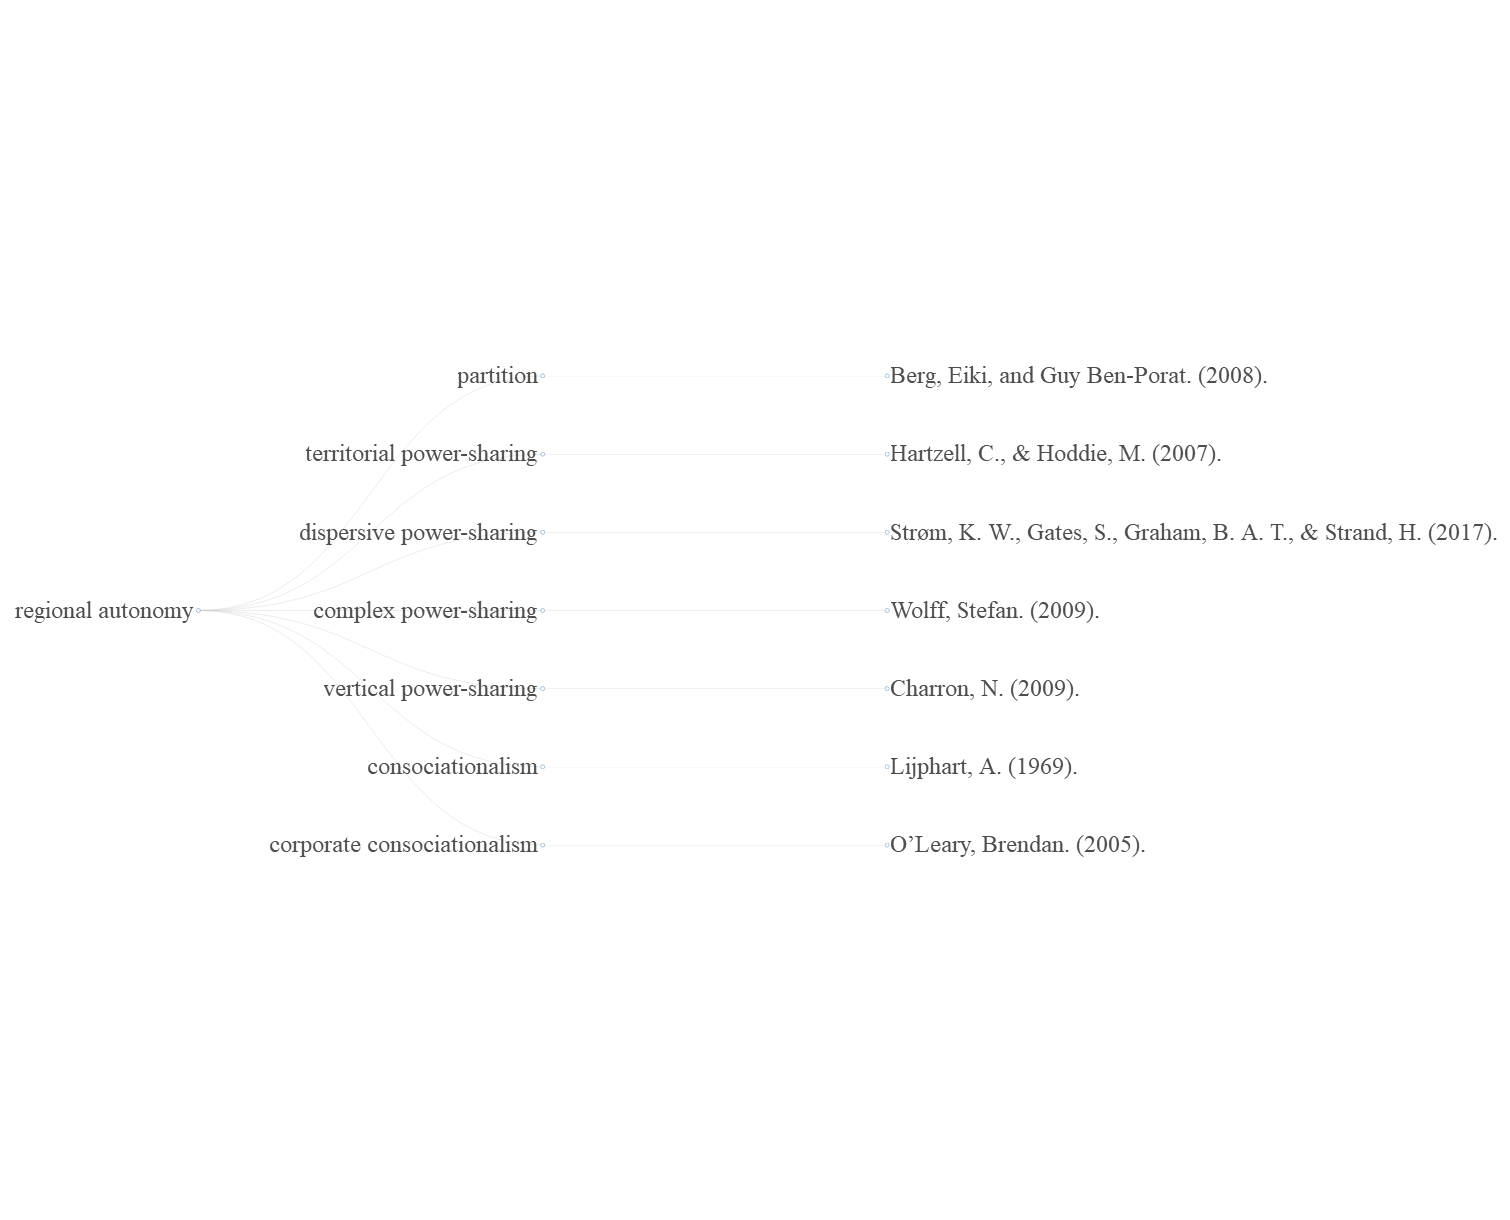
\includegraphics[width = 6in]{reg_aut_ontology_vis.png}
	\end{center}
\caption{Regional Autonomy Across Conceptualizations}
\end{figure}


This ontology could well be a significant development in the power-sharing literature. There are currently seventy-eight provisions when broken down by author, and yet these works often fail to highlight the relevance of the provisions themselves. I do not know whether all of the provisions of, say, coercive consociationalism or inclusive power-sharing, exert the same effect, whether some are redundant, or whether, when it comes to the institutionalization of peace, I face a simple case of ``more is better''. While these questions lie outside of the scope of this paper, I believe that a deeper analysis into the interactions of all known provisions---as opposed to the broader concepts themselves---will produce fascinating findings. 

While conducting the literature review portion of my thesis, I managed to extract most of the relevant information on the provisions of each form of power-sharing from the author’s typology tables. Further, authors who have conducted meta-analyses on power-sharing institutions such as Andeweg (2000), Bogaards (1998), and Norris (2008), include sections on the development of conceptions over time, allowing me to easily integrate terms into the ontology. Further, I have provided citations for each provision, and suggested a range of variables that could be utilized for measuring each provision. As mentioned, given that some of these provisions are inherently broad, not all provisions have been assigned a variable and, as such, unlock an avenue for further research. For pedagogical purposes, I have assigned upper-level nodes to be one of three possible parent classes: ``political systems'' such as liberal consociationalism, integrative consociationalism, and the like; ``power-sharing arrangements''---characterized as institutions implemented via peace agreements---such as territorial, economic, and military power-sharing; and ``power-sharing alternatives'' which encompass partition and power-dividing, concepts that are often posited in opposition to power-sharing institutions\footnote{The code and data for reproducing the ontology visualization can be found in the appendix of this paper.}.

To conclude, while there is much disagreement over the broad conceptions of power-sharing, analyzing the provisions of power-sharing make identifying causal mechanisms and outcomes far easier. It also allows for the reconciliation of conflicting studies on power-sharing. Segmental autonomy in particular is cited as a core provision across several conceptions of power-sharing, consociational democracy, and partition. Understanding this provision may serve to partially reconcile the power-sharing literature and provide insight into the causal mechanisms behind the implementation of power-sharing in ethnically divided and developing states. 

\section{Theory and Hypothesis}
States that employ segmental autonomy provisions along with other provisions of power-sharing, either through peace accord or constitutional reform, are more likely to experience reduced intergroup tensions and prolonged peace. That existing studies study segmental autonomy using different measures and do not isolate the individual effect of the variable, it is difficult to estimate what our results will show. That some authors argue in favor of consociationalism while others warn of its ineffectiveness, further muddies our theoretical prior. In an ethnically fractionalized state, where certain groups may have faced powerlessness or discrimination, the implementation of regional autonomy---be it through regional elections, educational authority, linguistic autonomy, or else---can be seen as a concession by the central government, and a signal of peace. Assuming this basic logic, I present my core hypotheses, and lay out a more nuanced theory and causal mechanism. 

\singlespacing

\textbf{H\textsubscript{1}}: Ethnically diverse states that employ segmental autonomy provisions, either through peace accord or constitutional reform, will experience reduced intergroup tensions, prolonged peace, and democratization.

\bigskip

\textbf{H\textsubscript{2}}: Ethnically diverse states that employ segmental autonomy provisions along with other provisions of power-sharing, either through peace accord or constitutional reform, will experience reduced intergroup tensions, prolonged peace and democratization. 

\doublespacing

Conversely, if my results do not confirm my hypothesis, I will fail to reject the null. 

\singlespacing

\textbf{H\textsubscript{Null}}: There will be no relation between the implementation of segmental autonomy provisions and the reduction in intergroup tensions, prolonged peace, and democratization in ethnically diverse states. 

\doublespacing

The causal chains that justify the implementation of segmental autonomy in ethnically diverse states come from the work of Lijphart (1969), Nordlinger (1972), and Esman (1973). They argue that provisions such as regional autonomy and other forms of power-sharing serve to ``reduce the long-range political salience of communal solidarities,'' though each embed this outcome in a slightly different framework\footnote{Esman, 1973, 55}. Moving beyond these broad theoretical arguments, I identify segmental autonomy operating in three distinct---but often overlapping---ways. 

\subsubsection{Proliferation of Focal Points}
Regional autonomy increases the number of political focal points in a state. By proliferating the number of autonomous regions, the central government can reduce the possibility of any one faction having power over another. As a result, the likelihood that one group feels disadvantaged or oppressed by another is reduced. Increasing the number of political focal points not only reduces inter-faction tensions, it also takes pressure off of the central government as the newly autonomous regions can act independently, such as by implementing their own tax, education, or language policies. Demands are thus less likely to be aimed at the central government, given that matters related to the ethnic group are in the hands of the subnational political bodies. We see the proliferation of subnational units in states such as Uganda and Nigeria as examples of a central government’s attempt to reduce the political salience of any given ethnic or regional group. The dispersive aspect of regional autonomy might reduce ethnic conflict and grievances by ``tak[ing] the heat off of a single focal point''\footnote{Horowitz, 1985, 598}. In dispersing political focal points and creating new outlets for political competition, regional autonomy might also allow the central government to consolidate power. Consolidation is particularly useful for new governments and governments in the midst of a conflict or political crisis. In these instances, regional autonomy essentially serves to draw attention away from the government, giving politicians manoeuvrability and allowing the central government to tighten their grip on the state through reconfiguring their power\footnote{Seely, 2001; Gasper, 1989}.

\subsubsection{Targeted Concessions to Regional Minorities}
The implementation of segmental autonomy provisions can serve as a concession to marginalized ethnic groups, potentially reducing the risk of conflict involving the central government or other ethnic groups. It is sometimes referred to as ``cooptation''\footnote{Seely, 2001}. In order to avoid the breakup of a state or a conflict, regional autonomy can abate political instability by meeting the needs of a dissatisfied group. As above, this can manifest as the group exerting substantial control over regional policymaking. One common argument against regional autonomy as a concession is that it opens the floodgates to more serious demands such as secession, and may increase ethnic violence. This is unlikely for two reasons. Firstly, secession itself is incredibly rare, and, whether successful or unsuccessful, secession is unlikely to be directly attributed to increased demands in autonomous locales\footnote{Mehler, 2013; Roeder, 2013}. Secondly, segmental autonomy is designed in part to balance any regional power disparities, and so additional demands are likely to come from groups who perceive themselves as being left behind. As Lluch (2012) argues, autonomism succeeds because of its hybridity and multiplicity: ``it can perfectly balance its anti-federalist stances with its grounding in the federalist principle of multiple levels of government within the same state apparatus, complemented by its anti-secessionism stance''\footnote{Lluch, 2012, 155}. When implemented thoughtfully, and when accounting for salient factions within a state, it is unlikely that forms of decentralization will lead to increased violence or calls for secession. 

\subsubsection{Checks and Balances on the Central Government}
Segmental autonomy is not just dispersive in nature. In ethnically fractionalized states in particular, segmental autonomy is most effective when it allows ethnic minorities to act independently of the central government while also giving that group some level of representation and control in the central government. Regional elections are a perfect example of such a mechanism. In implementing regional elections for geographically distinct ethnic minorities, previously powerless or discriminated groups are able to elect representatives of the same ethnic group who might them implement policies appropriate to the groups' needs. These elected members also serve as checks on the central government, thus legitimizing the regime. In granting more autonomy to salient regions, the central government might be perceived as more democratic and inclusive. Of course, attributing perceptions of democracy to the integration of regional actors into a central government is challenging to establish, but we do see decentralization improving public perceptions of democracy in various countries\footnote{Escobar-Lemmon and Ross, 2013; World Values Survey, 2007}. Beyond just perception, I believe that legitimization may in fact improve democracy given that regional actors, if integrated successfully, can serve as checks and balances on the central government.

\subsubsection{Alternative Mechanisms}
I also acknowledge some alternative theoretical arguments and potential threats of segmental autonomy. As mentioned, a common criticism of segmental autonomy is that it could lead to more aggressive demands, increased conflict, and potentially secession. The separation of groups along ethnic lines could reduce intergroup interactions to the point that prejudice and scapegoating may become the norm\footnote{Kelly, 2019}. Keller and Smith (2005) share a similar concern to Kelly (2019) in that segmental autonomy may go beyond political decentralization and group self-determination, instead exacerbating intergroup tensions and oppositional identities, and incentivizing more extreme concessions by the central government. They suggest that ``[t]he long-term implications of [subnational autonomy] are unclear, but in the short term there has been a tendency for increased demands for further autonomy among distinct groups within regions''\footnote{Keller and Smith, 2005, 240}. 

While these are issues that undoubtedly need to be considered during the planning and implementation of regional autonomy provisions, there are a number of issues with these claims. First, segmental autonomy is seldom a completely dispersive institution. As we have seen, provisions such as regional elections are both accommodative and integrative in nature, and so it is unlikely that ethnic groups will be partitioned to the point that they are unable interact with one another. Second, Keller and Smith (2005) use Ethiopia to argue against the effectiveness of segmental autonomy. Ethiopia is an interesting case given that there were calls for secession and hostile intergroup relations well before the implementation of ethno-federalism in 1991\footnote{Vogt et al., 2015}. Moreover, much of the ethnic conflict that followed the regional autonomy in 1991 arose because of the incomplete nature of its implementation. Certain ethnic groups were still discriminated, and the central government committed acts of violence against these marginalized groups\footnote{ibid.}. It is therefore important to supplement case studies with more rigorous empirical methods to avoid misleading extrapolation. In any case, ethnically fractionalized states with marginalized populations will, in some respect, benefit from increased autonomy and state recognition. The degree to which this is the case will be analyzed in Chapter 5.

\section{Segmental Autonomy in Mali and Niger}
The contiguous states of Mali and Niger provide an instructive qualitative comparison of the effects of regional autonomy. By process-tracing two well-matched countries, we are able to contextualize our theoretical mechanisms of autonomy and provide a plausible account of its effectiveness. As described in Table 2, the two states bear striking similarities at baseline that warrant further investigation and comparison: they have similar population sizes and GDP; share the same political system; and have both been subject to French colonial rule. More importantly, both states have a significant Tuareg population within their borders and similar ethnic group structures. According to their respective censuses, Mali comprises of 50\% Mande, 16\% Fula, 13\% Voltaic, and 10\% Tuareg while Niger consists of 55\% Hausa, 21\% Zarma-Songhai, and 9\% Tuareg. Though interethnic relationships between most groups are peaceful, the Tuaregs---who are more regionalized in Mali and Niger---have historically faced discrimination. The Tuareg are traditionally nomadic pastoralists, though in Mali and Niger they are largely regionally consolidated in the north. The Tuareg are linguistically and culturally distinct; they speak Tamasheq and, unlike other ethnic groups in Mali and Niger, are matrilineal. In addition to economic marginalization, the Tuareg have faced cultural discrimination such as the prohibition of nomadism in Niger and a lack of representation in the central government in both states\footnote{Ibrahim, 1994}. The Tuareg's violence toward the central government, and their demands for increased autonomy and representation, can be attributed to their shift between powerlessness and discrimination post-independence\footnote{Vogt et al., 2015}.  

Since independence in 1960, the two countries have had similar political experiences. From military and one-party rule for most of the 1960s and 1970s, to various coups d’état against autocratic leaders, to democratic reforms throughout the 1990s, Mali and Niger's stories have been of ethnic tension and regional instability. The two countries diverge significantly in 1999 when Mali, in response to growing ethnic tensions, implemented regional autonomy in the form of regional elections. Following similar ethnic violence and a coup, Niger opted for the inclusion of Tuareg members as ministers in a coalition government, and explicitly avoided regional autonomy provisions for the Tuareg population\footnote{Minorities at Risk Project, 2003}. In not implementing regional autonomy, various reports suggest that relations between the Niger government and the Tuareg ethnic population have declined, especially when compared to the relative peace and amicability between the Tuareg and the Malian government following autonomy. These well-matched cases allow for the use of John Stewart Mill's ``method of difference'' which compares different outcomes associated with an independent variable across two cases\footnote{Mill, 1843}. In Mali and Niger, the two states are also well-matched on the outcome variables prior to the implementation of segmental autonomy, where data exist. For example, both Mali and Niger ranked relatively low on the PolityIV index following independence and prior to democratization in the 1990s, and we see the two states diverge in purported levels of democracy and social trust ratings after 1999. For the other measures that these states have been matched on, Mali and Niger exhibit similar trends from independence through to the end of the century. This will be elucidated later in the section, but these similar characteristics and parallel trends on the variables and outcomes of interest provide justification to process-trace the impacts of segmental autonomy. 

\begin{table}[!htbp]
	\centering
	\setlength{\tabcolsep}{10pt}
	\renewcommand{\arraystretch}{1.5} 
	\resizebox{\textwidth}{!}{\begin{tabular}{|l|c|c|}
			\hline
			\textbf{Country}                &   \textbf{Mali}  &  \textbf{Niger}  \\ 
			\hline
			Regional Autonomy?              &   Yes            &  No              \\
			\hline
			Population (1999, millions)     &   10.6           &  10.9            \\
			\hline
			Tuareg \% of Population (2001)  &   10             &  9.3             \\
			\hline
			GDP (1999, billion USD)         &   3.4            &  2.0             \\
			\hline
			Ethnic Fractionalization (1999) &   0.8            &  0.6             \\
			\hline
			Area (million sq. km.) 			&   1.2 		   &  1.3 			  \\
			\hline
			Former French Colony?			&  Yes			   &  Yes			  \\
			\hline 
			Political System                &  Unitary semi-presidential republic & Unitary
			semi-presidential republic  \\
			\hline
	\end{tabular}}
	\caption{Country Characteristics Around Mali's Decentralization}
\end{table}

Prior to achieving autonomy in 1999, the Tuareg had been pressuring the Malian government to decentralize decision-making and grant them greater economic freedom. Though the Malian government were concerned that the Tuareg might push for a complete secession from the state, they refused to grant the Tuareg people regional autonomy or any form of power-sharing provision\footnote{Girardin et al., 2015}. Students and civil servants began protesting in January of 1991 as a result of persistent economic decline and oppressive rule\footnote{The New York Times, 1991; The Los Angeles Times, 1991}. Exacerbated by Tuareg pressures to devolve powers, these protests culminated in a coup d’état in March of 1991 against authoritarian leader Moussa Traoré. The following year saw the introduction of peace accords granting the Tuareg some level of regional autonomy\footnote{Humphreys, 2005}. Though intended to abate tensions between the central government and the ethnic groups in Mali, the peace accords were not fully implemented until 1999 when the first Tuareg regional elections were held\footnote{Keita, 1998; Seely, 2001}. Prior to the regional elections, rates of politically-motivated conflict between the Tuareg, the central government, and other minority ethnic populations, remained high. In the years following the \textit{de facto} implementation of regional autonomy, conflict rates and fatalities appeared to decrease. The Ethnic Power-Relations Atlas (EPR) anecdotally remarks that following regional autonomy in the north east, conflict rates markedly decreased, especially within the Tuareg region\footnote{Vogt et al., 2015}. Similarly, the Minorities at Risk Project notes that, despite a recent history of rebellion and violence, Mali's Tuareg population are ``unlikely to engage in large-scale violence in the near future'' as the government has provided, through decentralization ``more openings for conventional and nonviolent political activity''\footnote{Minorities at Risk Project, 2003}. 

The Tuareg in Niger faced similar discrimination post-independence. As in Mali, the Tuareg were economically marginalized and effectively unable to participate in government decision-making. In 1993, two years after especially intense violence between the military government and the Tuareg population, a power-sharing government was established in the form of a coalition cabinet. Though some government positions were held by Tuareg politicians, they were quickly sacked and detained\footnote{Krings, 1995}. It was not until 1994 that the Tuareg---though still in the midst of violence with state army---were successfully integrated into the governing coalition. While their inclusion pointed to reduced tensions, 2004 saw the removal (and execution) of Tuareg officials in government, effectively ending the coalition cabinet model of power-sharing. Again, the Tuareg were rendered powerless, and in 2007 a Tuareg rebellion broke out against the government demanding more representation. Interestingly, the 2007 Tuareg rebellions occurred in both Mali and Niger almost simultaneously, but where the violence in Mali focused on the government's failure to implement economic reforms, the violence in Niger was attributed to their political exclusion\footnote{Bertelsmann, 2008}. 

Why did the Nigerien government refuse decentralization? Pons (1993) argues that the regions populated by the Tuareg happen to be rich in uranium, which, during the 1990s, accounted for about 80\% of Niger's exports. The central government did not wish to relinquish their most economically viable region to an ethnic minority and adversary and thus sought integration through alternative power-sharing provisions\footnote{Krings, 1995; Pons 1993}. These provisions were never fully realized and, as a result, the Tuareg population in Niger---throughout the numerous democratic and authoritarian transitions since 1999---are purported to exhibit several risk factors for rebellion and increased violence\footnote{Minorities at Risk Project, 2003}. 

Recall that segmental autonomy might reduce conflict through serving as a concession to marginalized and dissatisfied ethnic groups, and legitimize a regime by giving minority groups more policymaking power and political representation. There exists evidence of autonomy's positive cooptive effect as, immediately after the implementation of autonomy, Tuareg rebels willingly ``handed over mortars, anti-tank mines and grenade launchers'' to the central government, who then destroyed these weapons\footnote{Reuters, 2008}. This ceremonial event shows that the implementation of regional autonomy was a concession made by the central government to the Tuareg minority in a bid to reduce conflict. Empirically, little work has been conducted to assess whether the number of casualties has changed since the implementation of autonomy in Mali, though data from the Armed Conflict Location and Event Data (ACLED) indicates that the implementation of segmental autonomy was a contributing factor to the reduction of conflict\footnote{Raleigh et al., 2010};\footnote{Brailey, 2019, unpublished manuscript}. Perhaps more importantly, regional autonomy also served to legitimize the Tuareg, who were represented in the central government following the regional elections in 1999. Evidence suggests that perceptions of democracy improved following the implementation of regional autonomy and several rounds of successful regional elections in northern Mali\footnote{World Values Survey, 2007}.

In process-tracing the political histories and trajectories of post-independence Mali and Niger, it is clear that Niger has faced greater political unrest as a result of dictatorial leadership (such as the constitutional crisis of 2009), economic and environmental factors, and other factors unrelated to the power-sharing institutions themselves. However, it is undeniable that much of the ethnic unrest and violence stems directly from the central government's inability to meaningfully integrate or accommodate the Tuareg population. This includes their failure to grant regional autonomy to the Tuareg after several decades of Tuareg demands. While the political future of the Tuareg in Mali is uncertain and conflict persists as a result of underlying economic grievances, the level of violence between ethnic minorities and the central government is far less severe than in Niger.

As with the empirical conceptions of regional autonomy, \textit{prima facie} evidence from Mali and Niger should be interpreted with caution and two caveats are in order. First, though this paper seeks to understand the impacts of regional autonomy across three dimensions---conflict, social and intergroup trust, and democratization---evidence and measurements for the latter two variables in the two states are scarce. Afrobarometer data exists for Mali in 2000, and suggests that there is broad support for democracy and a general satisfaction with democratic institutions\footnote{Afrobarometer Data, Mali, Round 1, 1991, available at http://www.afrobarometer.org.}. While these data support the findings of existing studies, that no pre-autonomy measures of these variables exist makes establishing causal or correlative relationships essentially impossible. Second, we see that these states are facing a plethora of dynamic political issues, making it difficult to isolate and attribute a single causal mechanism. To elucidate, if regional autonomy is in fact reducing intergroup tensions, there exists little data to analyze ethnic group trust for the Malian population in and around 1999, and even if the data did exist it would be difficult to isolate regional autonomy as the main cause, given that there are several other country-specific factors operating and interacting with autonomy and its implementation. It is worth mentioning the resource curse as one such country-specific factor in Niger. A large body of literature suggests that, because Niger relied on uranium as its primary export, the state is inherently more likely to face political instability and autocratic shifts\footnote{Mehlum et al., 2006; Sachs and Warner, 2001}. While this may have contributed to Niger's overall instability, Tuareg violence occurred irrespective of resources; their focus was solely on achieving more political influence. In any case, evidence from Mali and Niger, and the seemingly positive impacts of regional autonomy in the former state, warrants further investigation as to the substantive effects of regional autonomy in ethnically fractionalized polities. 

\section{Methodology}
\subsection{Data Collection}
Data collection began with a broad overview of existing datasets on power-sharing in existing papers. A great deal of time was spent finding and reading-in the data, as well as reaching out to academics in order to find codebooks and bypass dead weblinks. As mentioned, Ansorg et al.’s (2013) expansive study on existing datasets was of great help in my own evaluation of existing datasets. Their findings very much parallel my own experiences with these political datasets: they are often hard to obtain; they often do not contain all the information required to fully understand the data; they are often conceptualized and parameterized differently, making comparison especially challenging; and there is often little information on how the variables were coded, reducing the credibility of these data. Moreover, many of the datasets suffer from significant missingness, again potentially reducing the accuracy of the authors’ findings. As mentioned, I create a unique ontological dataset on the provisions of power-sharing based off of the literature review. It contains the core provisions of power-sharing, power-dividing, and partition, the source author, and any variables that relate to the provisions. After identifying datasets that contained variables or potential proxies for the provisions that have been conceptualized in the literature, I merge them to create a second unique dataset\footnote{See the appendix at the end of this paper for the code to replicate the ontology.}. I use Strøm et al.’s (2017) ``Inclusion, Dispersion and Constraint Dataset'' as it is arguably the most complete dataset on power-sharing provisions---despite only covering data from 1975 through to 2010. Other datasets included in the final merge are Norris (2008), Hartzell and Hoddie (2007), and Jaarstad and Nilsson (2008), as well as datasets from the Database of Political Institutions, Varieties of Democracy, Quality of Governance, and Ethnic Power-Relations. I elaborate on the nature of the data and future endeavors in the scope and limitations section of the paper\footnote{It should be noted that all the code written for this project have been formatted as R Markdown files and can be found in the appendix of this paper.}.  

Given that many of the prominent datasets have high percentages of missingness, this is something that has to be accounted for in my own analyses. Where possible, I have filled out missing observations for the variables used in my statistical analysis and summary plots. Visualizations of the merged data’s missingness can be found in the appendix. 

\subsection{Measurements}
\subsubsection{Dependent Variables} 
In my attempt to partially reconcile the literature on power-sharing, I run statistical tests on three main dependent variables and several supplemental dependent variables. I use QOG’s hum\_trust variable to measure the effect that the implementation of segmental autonomy has on a social trust. hum\_trust is an index score which represents an average of all country-survey scores available within each country-year and is measured from 0—no social trust—to 100—complete trust in others. I also use the hum\_satdem and hum\_supdem in QOG as supplements to measure whether satisfaction or support for democracy changes with the implementation of segmental autonomy provisions. These are also indices of survey data on the country-year level. My second dependent variable is the PolityIV project’s polity score, a twenty-one-point score that captures a state’s level of democracy, anocracy, or autocracy. In line with my core hypothesis, I use this variable to understand whether there is a statistically significant relationship between the presence of regional autonomy and changes in democracy. My final dependent variable comes from the Uppsala Data Conflict Program (UCDP) and addresses the relationship between conflict rates and autonomy. I utilize a binary and continuous measurement of state conflict for robustness. The binary variable captures whether, in a given country-year observation, there were over one-thousand battle deaths, while the continuous variable captures the severity of that conflict by the number of deaths, with fewer than one-thousand being considered minor, and over one-thousand being considered a war. 

\subsubsection{Independent Variables} 
My core independent variable is the implementation of segmental autonomy. I utilize other dataset’s conception of autonomy as well as my own variable for robustness. In all cases, the measurement of autonomy is dichotomous. Firstly, I use the \textit{auton} variable found in Strøm et al.’s (2017) Inclusion, Dispersion, and Constraint dataset, and the DPI database. DPI conceptualizes the measurement as follows:

\singlespacing
Autonomous regions are not the same as states, provinces, etc. An autonomous region is recorded if a source explicitly mentions a region, area, or district that is autonomous or self-governing. Furthermore, they must be constitutionally designated as ``autonomous'' or ``independent'' or ``special''. Federal Districts or Capital Districts do not count as autonomous regions. Disputed autonomy is not recorded. Indian reservations are not counted as autonomous. \textbf{Deviating from convention, no information recorded as 0}\footnote{Cruz et al., 2018, emphasis in original}.

\doublespacing
I supplement these core assessments of the presence of autonomous regions by running simple bivariate regressions using different measures of regional autonomy from Ethnic Power Relations and the Regional Autonomy Index. Though I have already assessed the correlation between these variables, it seems logical to assess their predictive power with regards to our outcome variables of interest. The results of these bivariate regressions can be found in the results section. 

\subsubsection{Control Variables} 
The impetus behind including my control variables comes from existing empirical studies\footnote{Hartzell and Hoddie, 2007; Kelly, 2019; Norris, 2008; Strøm et al., 2017; Walter, 2002} and the necessity of country controls. As such, I have included variables from QOG on political stability, the Gini Index, population, and polity score\footnote{I exclude polity score from the model where the dependent variable is also polity score}. Additionally, I calculate a new variable, tb\_other\_provis, which takes a value of one when any of the other core provisions of consociational democracy---mutual veto, proportionality, or grand coalition---are present in any country-year observation, and use this to calculate interaction effects in my models. 

\subsection{Empirical Conceptions of Segmental Autonomy}
While it is important to understand the substantive effects that provisions of power-sharing exhibit when implemented, an equally important question is how the field operationalizes these concepts and whether these measures can be considered construct valid. As such, I utilize measurements of constructs from four different datasets in order to better understand the construct validity of regional autonomy. These datasets include DPI\footnote{Cruz et al., 2015}, Ethnic Power Relations (EPR)\footnote{Vogt et al., 2015}, Inclusion, Dispersion, and Constraint (IDC)\footnote{Strøm et al., 2015}, and the Regional Autonomy Index (RAI)\footnote{Hooghe et al., 2015}. The Local Autonomy Index\footnote{Ladner et al., 2019} and PA-X\footnote{Bell et al., 2019} measurements are not included in the analysis given that their units of analysis cannot easily be manipulated to align with the other datasets. Based on the codebook descriptions for these variables, we expect the autonomy variables (\textit{auton}, \textit{n\_RAI}, and \textit{reg\_aut}) to exhibit high correlation amongst one another and low correlation between constructs that are theoretically different (\textit{author}, \textit{subtax}, \textit{subed}, and \textit{subpolice}). Table 1 shows Pearson correlations for these variables.

Intuitively, among measures of subnational authority (\textit{subtax}, \textit{subed}, \textit{subpolice}, \textit{author}), we see relatively high levels of correlation (0.65 - 0.81). Less intuitively, however, among the three measures of regional autonomy, there is relatively low correlation across all three models (0.24 - 0.41). We also see \textit{n\_RAI} correlate highly with measures of subnational authority, between which we should theoretically be able to distinguish. These findings hearken back to Adcock and Collier's (2001) discussion on establishing equivalence across context-specific observations\footnote{Adcock and Collier, 2001, 534-535}. In other words, different country-specific contexts make generalized measurements especially difficult, exemplified by the fact that three supposedly theoretically convergent constructs have been operationalized in such a way so as to be weakly correlated with one another and more strongly correlated with theoretically and conceptually different constructs.

Where does this leave us? Frustratingly, the development of a new measurement that seeks to reconcile existing conceptions of regional autonomy is beyond the scope of this paper. Instead, these findings necessitate heightened caution and care when drawing inferences and making conclusions based on statistical results. Regional autonomy is not---as we saw with the debate on consociationalism---a well-defined concept, and the implications of which must be addressed in my methodology. Section 5 will address these conceptual discrepancies from an empirical standpoint. 

\begin{table}[ht]
	\centering
	\setlength{\tabcolsep}{4pt}
	\renewcommand{\arraystretch}{1.5} 
	\resizebox{\textwidth}{!}{
		\begin{tabular}{rlllllll}
			\hline
			& \textit{auton} (DPI) & \textit{n\_RAI} (RAI) & \textit{reg\_aut} (EPR) & \textit{subtax} (IDC) & \textit{subed} (IDC) & \textit{subpolice} (IDC) & \textit{author} (DPI) \\ 
			\hline
			\textit{auton} (DPI) & 1 &  &  &  &  &  &  \\ 
			\textit{n\_RAI} (RAI) & 0.24 & 1 &  &  &  &  &  \\ 
			\textit{reg\_aut} (EPR) & 0.32 & 0.41 & 1 &  &  &  &  \\ 
			\textit{subtax} (IDC) & 0.20 & 0.86 & 0.46 & 1 &  &  &  \\ 
			\textit{subed} (IDC) & 0.15 & 0.7 & 0.35 & 0.78 & 1 &  &  \\ 
			\textit{subpolice} (IDC) & -0.05 & 0.83 & 0.35 & 0.76 & 0.65 & 1 &  \\ 
			\textit{author} (DPI) & 0.18 & 0.79 & 0.38 & 0.77 & 0.65 & 0.81 & 1 \\ 
			\hline
	\end{tabular}}
	\caption{Pearson's Correlation of Segmental Autonomy and Authority Measurements}
\end{table}

\subsection{Models}
Prior to running statistical models, I generate simple cross-sectional time-series plots that show the relationship between the percentage of years each state has spent with \textit{de jure} implementation of segmental autonomy and levels of social trust, polity score, and conflict intensity within the state. These summary statistics can be found in the appendix of this paper. As these cross-sectional visualizations include all states in the dataset, we do not see any significant trends across time, though it does give some insight into how prevalent segmental autonomy is across the world's states. 

I begin my statistical analyses by subsetting the data to those states that exhibit high levels of ethnic fractionalization (characterized by states that have an ethnic fractionalization score of above the world median value), and then running several iterations of robust ordinary least squares (OLS) regression on my cross-sectional time-series dataset on three distinct dependent variables. For conflict duration as a dependent variable, I run a Cox proportional hazards model to assess whether the implementation of regional autonomy serves to reduce the length of a conflict. For each dependent variable---levels of social trust, conflict intensity, and polity score---the same control variables are included in the OLS. For all models, I include country fixed-effects, and for the latter two iterations, I include year fixed-effects. Lastly, to ensure my estimates are robust, the OLS regressions are clustered by standard error.  

\section{Results}
The three core models provide some convincing evidence for my hypotheses. I start by analyzing my OLS and Cox model results and then move into assessing measurements of regional autonomy and robustness checks. Table 3 shows the impact of segmental autonomy on social trust levels for all country-year observations that fall above the median ethnic fractionalization value for all states in my dataset. Here, social trust is taken to be the average of all country-survey scores available within each country-year observation, with 0 representing the lowest possible trust levels, and 100 representing the highest possible trust levels. The results are mixed. The first hypothesis posits that regional autonomy, in granting ethnic groups more political power and serving as a concession to marginalized ethnic groups, reduces political grievances and intergroup tensions. A simple bivariate regression indicates that regional autonomy exerts a statistically significant positive effect on levels of social trust across states, however, the inclusion of control variables and year fixed effects flips the direction of regional autonomy---from a 0.4-point increase to a -30.8-point decrease---and renders it not statistically significant. We see that the presence of other consociational provisions exert a negative and statistically insignificant effect on levels of social trust in a state, though this becomes positive and significant at the ten-percent level when we interact this variable with the regional autonomy measure. The adjusted $R^2$ values across models suggest that the Model 3 is able to explain up to 51\% of the total variance in the data, though there is not much change in the $R^2$ and adjusted $R^2$ values across models. Similarly, the root mean squared error (RMSE)---standard deviation of the unexplained variance---does not differ significantly across models, indicating that additional control variables do not better explain the variation in the outcome variable.  

\begin{table}[!htbp]
	\begin{center}
		\begin{tabular}{l c c c }
			\hline
			& Model 1 & Model 2 & Model 3 \\
			\hline
			(Intercept)                  & $49.65^{***}$ & $22.38$   & $22.38$     \\
			& $(0.00)$      & $(12.09)$ & $(12.09)$   \\
			Regional Autonomy                   & $0.40^{***}$  & $-30.83$  & $-30.83$    \\
			& $(0.00)$      & $(23.94)$ & $(23.94)$   \\
			Political Instability               &               & $4.89$    & $4.89$      \\
			&               & $(5.03)$  & $(5.03)$    \\
			Gini Index               &               & $0.49$    & $0.49$      \\
			&               & $(0.32)$  & $(0.32)$    \\
			Population               &               & $0.00$    & $0.00$      \\
			&               & $(0.00)$  & $(0.00)$    \\
			Polity Score       &               & $0.77$    & $0.77$      \\
			&               & $(0.82)$  & $(0.82)$    \\
			Other Provisions           &               & $-12.28$  & $-12.28$    \\
			&               & $(3.39)$  & $(3.39)$    \\
			Regional Autonomy:Other Provisions &               &           & $29.00^{*}$ \\
			&               &           & $(5.98)$    \\
			\hline
			Country Fixed Effects?		 & Y			 & Y 		   & Y			  \\
			Year Fixed Effects?			 & N			 & Y		   & Y			  \\
			R$^2$                        & 0.51          & 0.58      & 0.58        \\
			Adj. R$^2$                   & 0.47          & 0.51      & 0.51        \\
			Num. obs.                    & 598           & 409       & 409         \\
			RMSE                         & 11.47         & 11.53     & 11.53       \\
			\hline
			\multicolumn{4}{l}{\scriptsize{$^{***}p<0.001$, $^{**}p<0.01$, $^*p<0.05$}}
		\end{tabular}
		\caption{Segmental Autonomy's Effect on Social Trust}
		\label{table:coefficients}
	\end{center}
\end{table}
			
The second hypothesis posits that regional autonomy---again serving as a concession to marginalized and potentially de-stabilizing groups---reduces conflict in ethnically fractious regions. Table 4 uses a dichotomous conflict measurement as the dependent variable; it takes a value of 1 when there is a significant conflict occurring in a given year, and 0 otherwise\footnote{UCDP defines ``significant'' as a conflict with over 1000 battle-related deaths. For the purposes of this study, the value is subsetted to only internal conflicts. A number of issues arise with this coding of conflict and they will be addressed in a later section.}. Again, we do not see segmental autonomy exert any statistically significant effect on conflict intensity levels in ethnically diverse states. Similar to the results in our OLS on social trust levels, the interaction effect between regional autonomy and other consociational provisions serve to reduce conflict to a statistically significant degree. The Cox model indicates that these variables reduce conflict by a factor of 47\%\footnote{Cox regression models calculate the association between ``survival'' time and a given independent variable. Here, a hazard ratio coefficient of 0.53 reduces the hazard by 47\%.}. Though this is only weakly statistically significant, these findings do provide some evidence that the presence of autonomy, when implemented alongside other provisions of power-sharing, may reduce conflict rates in ethnically diverse polities. 

\begin{table}[!htbp]
	\centering
	\begin{tabular}{lrrrr}
		\hline
		& coef & HR = exp(coef) & 95\% CI & $p$-value \\ 
		\hline
		Regional Autonomy & 0.38 & 1.47 & [0.83, 2.59] & 0.19 \\ 
		Other Provisions & 0.58 & 1.79 & [1.20, 2.67] & $0.00^{**}$ \\ 
		Political Instability & -0.04 & 0.96 & [0.77, 1.20] & 0.73 \\ 
		Gini Index & 0.00 & 1.00 & [0.98, 1.03] & 0.79 \\ 
		Population & -0.00 & 1.00 & [1.00, 1.00] & 0.49 \\ 
		PolityIV Score & -0.02 & 0.98 & [0.95, 1.01] & 0.20 \\ 
		Regional Autonomy:Other Provisions & -0.64 & 0.53 & [0.25, 1.12] & $0.10 {\textbf{ .}}$ \\ 
		\hline
		\multicolumn{4}{l}{\scriptsize{$^{***}p<0.001$, $^{**}p<0.01$, $^*p<0.05$, $\textbf{.}p<0.1$}}
	\end{tabular}
	\caption{Cox regression model, $n = $ 245, number of events = 195.} 
	\label{mod}
\end{table}

Perhaps the most compelling finding of this study is the effect that the presence of segmental autonomy has on democratization in an ethnically fractionalized state, as shown in Table 5. Recall that segmental autonomy can serve to legitimize a regime by granting power to a diverse range of actors, and that legitimization may extend from just positive perceptions of democracy to actual improvements of democratic performance. Using PolityIV polity score, a twenty-one point index of democratic indicators, we can assess the substantive effects of regional autonomy. Across all three models, the implementation of segmental autonomy correlates with increased polity scores, and when accounting for control variables and interaction effects, the statistical significance of the presence of segmental autonomy increases. Somewhat counterintuitively, the interaction effect between regional autonomy and other consociational provisions reduces democracy levels with weak statistical significance. This will be discussed in the following section. 

\begin{table}[!htbp]
	\begin{center}
		\begin{tabular}{l c c c }
			\hline
			& Model 1 & Model 2 & Model 3 \\
			\hline
			(Intercept)                  & $-7.27^{***}$ & $-4.07$  & $-4.07$       \\
			& $(0.00)$      & $(2.96)$ & $(2.96)$      \\
			Regional Autonomy                  & $2.94$        & $0.24$   & $11.53^{***}$ \\
			& $(3.67)$      & $(1.55)$ & $(1.69)$      \\
			Political Instability              &               & $0.87$   & $0.87$        \\
			&               & $(0.65)$ & $(0.65)$      \\
			Gini Index              &               & $0.02$   & $0.02$        \\
			&               & $(0.05)$ & $(0.05)$      \\
			Population                &               & $0.00$   & $0.00$        \\
			&               & $(0.00)$ & $(0.00)$      \\
			Other Provisions           &               & $0.65$   & $0.65$        \\
			&               & $(0.77)$ & $(0.77)$      \\
			Regional Autonomy:Other Provisions &               &          & $-6.20^{*}$   \\
			&               &          & $(2.67)$      \\
			\hline
			Country Fixed Effects?		 & Y			 & Y 		   & Y			  \\
			Year Fixed Effects?			 & N			 & Y		   & Y			  \\
			R$^2$                        & 0.64          & 0.82     & 0.82          \\
			Adj. R$^2$                   & 0.63          & 0.79     & 0.79          \\
			Num. obs.                    & 2379          & 758      & 758           \\
			RMSE                         & 4.27          & 2.35     & 2.35          \\
			\hline
			\multicolumn{4}{l}{\scriptsize{$^{***}p<0.001$, $^{**}p<0.01$, $^*p<0.05$}}
		\end{tabular}
		\caption{Segmental Autonomy's Effect on Democratization}
		\label{table:coefficients}
	\end{center}
\end{table}

\section{Discussion} 
The OLS and Cox regression models provide some convincing evidence in support of my hypotheses. Regarding levels of social trust, we see segmental autonomy provisions alone having no significant effect, though we do see the presence of multiple consociational provisions increasing levels of social trust with statistical significance. However, the high RMSE value and $R^2$ value purports to only explain fifty percent of the variance in the relationship between autonomy and social trust, and so even when account for country and year fixed-effects and our controls, these core provisions fail to explain the underlying patterns in the data. While I will elucidate further in the next section, issues such as a lack of data when controlling for all independent variables may indeed have affected my results. These results could also be function of our measure of social trust, which does not have complete country coverage and is an index of existing surveys rather than an exact measure. Though it provides the best coverage overall, future research should focus on aggregating fine-grain, cross-country, survey data focusing specifically on attitudes toward fellow ethnic groups pre- and post-decentralization. 

Similarly interesting results emerge when evaluating conflict. As discussed, we see that regional autonomy plus a mix of other consociational provisions---either mutual veto, grand coalition, or proportionality---reduces conflict rates by a factor of 47\%, while regional autonomy alone does not seem to exert a statistically significant effect either way. Of course, different measures of conflict could be used to assess this hypothesis, but a simple binary provides sufficient evidence of the potential of segmental autonomy when employed alongside other provisions.  

The final dependent variable, polity score, seems to correlate well with the presence of segmental autonomy. As mentioned, it does seem counterintuitive for more power-sharing provisions to exert a negative effect, though I identify two possible explanations. First, ethnically fractionalized and conflictual polities, ones which inherently register low on PolityIV's index, may attempt to implement broader consociational institutions. Examples of this include Iraq's 2004 constitution and the Addis Ababa Agreement in Sudan in 1972. Second, including an interaction effect reduces the number of observations in a regression, and so these results could be a function of a lower $N$ rather than a substantive effect of the interaction. That said, the high adjusted $R^2$ values and relatively low RMSE values suggest that these models do a good job of predicting the outcomes and explaining the variance within the data. The results presented in Table 5 are especially compelling given that country fixed effects and clustered standard errors are designed to account for any possible confounding variables and alternative explanations. The fact that such a strong relationship exists across the two multivariate regressions in spite of the threat of type II error suggests that the effect of regional autonomy on democracy scores is salient. 

\subsection{Robustness Checks}
One potential alternative explanation to the results in Table 5 is that decentralization could be a component of the polity score index. In other words, if PolityIV incorporate regional autonomy into their measure of polity score, my dependent and independent variables would be fundamentally the same and would thus be perfectly correlated. To account for this, I run the same regression as in Table 5, but swap out the dependent variable for a measure of free and fair elections in Table 6. This variable comes from V-Dem, and asks: ``Taking all aspects of the pre-election period, election day, and the post-election process into account, would you consider this national election to be free and fair?''\footnote{Coppedge et al., 2018} It is an ordinal variable where 0 indicates the election was not free or fair, and 4 indicates that the election was free and fair. Logically, we see that polity score is correlated with free and fair elections, given that the latter is a component of the former. More interestingly, we see that, as with the results in Table 5, the presence of regional autonomy increases free and fair elections by 1.8 points and is statistically significant at the p $<$ 0.001 level. The presence of other consociational provisions also increases democracy when using this measure as a proxy. These results suggest that, irrespective of our measure of democracy, the implementation of regional autonomy serves to improve democracy in ethnically fractious regions. One final point: the interaction effect of regional autonomy and other provisions, is, as was the case in the previous model, negatively associated with democracy, though it is statistically insignificant. This seems to be at odds with Norris (2008) who suggests that the more power-sharing provisions implemented, the better. As mentioned, this could simply be a function of the inherent characteristics of states where regional autonomy is employed, or of a lower $N$ compared to the preceding models.  

\begin{table}[!htbp]
	\begin{center}
		\begin{tabular}{l c c c }
			\hline
			& Model 1 & Model 2 & Model 3 \\
			\hline
			(Intercept)                  & $-1.39^{***}$ & $-0.64$     & $-0.64$      \\
			& $(0.00)$      & $(0.64)$    & $(0.64)$     \\
			Regional Autonomy                   & $0.04$        & $-0.50$     & $1.80^{***}$ \\
			& $(1.56)$      & $(0.33)$    & $(0.36)$     \\
			Political Instability               &               & $0.04$      & $0.04$       \\
			&               & $(0.08)$    & $(0.08)$     \\
			Gini Index              &               & $0.00$      & $0.00$       \\
			&               & $(0.01)$    & $(0.01)$     \\
			Population               &               & $-0.00$     & $-0.00$      \\
			&               & $(0.00)$    & $(0.00)$     \\
			Polity Score       &               & $0.05^{**}$ & $0.05^{**}$  \\
			&               & $(0.01)$    & $(0.01)$     \\
			Other Provisions            &               & $0.41^{*}$  & $0.41^{*}$   \\
			&               & $(0.15)$    & $(0.15)$     \\
			Regional Autonomy:Other Provisions &               &             & $-0.22$      \\
			&               &             & $(0.29)$     \\
			\hline
			Country Fixed Effects?		 & Y			 & Y 		   & Y			  \\
			Year Fixed Effects?			 & N			 & Y		   & Y			  \\
			R$^2$                        & 0.69          & 0.92        & 0.92         \\
			Adj. R$^2$                   & 0.68          & 0.91        & 0.91         \\
			Num. obs.                    & 2111          & 753         & 753          \\
			RMSE                         & 0.81          & 0.36        & 0.36         \\
			\hline
			\multicolumn{4}{l}{\scriptsize{$^{***}p<0.001$, $^{**}p<0.01$, $^*p<0.05$}}
		\end{tabular}
		\caption{Alternative Measure to PolityIV Score (Free and Fair Elections)}
		\label{table:coefficients}
	\end{center}
\end{table}

Table 7 provides an assessment of the different measures of autonomy's predictive validity. As discussed, much of the existing power-sharing literature purports that autonomy will either have a null or positive effect on democratization\footnote{Lijphart, 1969; Lijphart, 1975; Nordlinger, 1974; Norris, 2008; Kelly, 2019; Rothchild and Roeder, 2005}. This is through the generation of multiple focal points that simultaneously reduces political pressure on the central government while also legitimizing the regime. When I take the most demanding regression model from the main results section---incorporating clustered standard errors, country and year fixed effects, and control variables---and use PolityIV's polity score measurement as the dependent variable, I find that each measurement exerts a completely different effect on polity score. The Ethnic Power Relations measurement of regional autonomy (which, like DPI's measurement, is a binary variable) suggests that the presence of regional autonomy in ethnically diverse states exerts a weakly negative and statistically insignificant effect on democratization. Similarly, the Regional Autonomy Index variable exerts a negative and statistically insignificant effect on democratization. Both alternative measurements remain insignificant when interacting with other consociational provisions, leading to questions of construct validity. These findings seem to be in line with the core of my argument. Recall that the simple correlation table suggested that measures of regional autonomy were not well correlated with each other, whereas measures of subnational authority (a distinct but theoretically related concept) showed much higher correlation rates across different measurements. Given that existing measures of regional autonomy are not well correlated, it seems logical that we would see contrasting results in our regression model.

How do we reconcile this disconnect? To start, is worth noting that the Regional Autonomy Index does not have the same country-coverage as the DPI and EPR measures, so it is likely that the discrepancy in results is due to this difference in coverage. RAI is also a bounded continuous rather than a binary variable, which could also contribute to the differing results across measurements. The discrepancy between DPI's and EPR's measurement is a little harder to pin down, though it is most likely related to three distinct features of the dataset: the unit of analysis, and the broader conceptualizations of ethnic groups and of regional autonomy. Given that EPR's unit of analysis is country-year-ethnic group, there is more fine-grain information on regional groups and their power-relations. EPR's codebook states that an ethnic group is included in the dataset ``if either at least one significant political actor claims to represent the interests of that group in the national political arena or if group members are systematically and intentionally discriminated against in the domain of public politics''\footnote{Vogt et al., 2015}. This conception has far greater coverage of ethnic groups compared with DPI, and as their regional autonomy measure is based on each coded ethnic group, there are more recorded instances of regional autonomy overall. Lastly, EPR's conception of regional autonomy specifies different state levels of autonomy as well as types of autonomy---language, education, tax, and spending---and thus contains more cases of autonomy. Here we get to the root of the issue, the Inclusion, Dispersion, and Constraint, dataset uses DPI's measurement for regional autonomy and supplements it with measures of subnational tax, education, and police autonomy, suggesting that regional autonomy and regional authority are different concepts. Put differently, EPR's measure of regional autonomy amalgamates autonomy and authority, reducing the construct validity of the measure. In sum, these results suggest that, even with the use of indices and other aggregate measurements, the concept of regional autonomy is difficult to pin down. 

\begin{table}[!htbp]
	\begin{center}
		\begin{tabular}{l c c c }
			\hline
			& Model 1 & Model 2 & Model 3 \\
			\hline
			(Intercept)                          & $-4.07$       & $-4.23$  &          \\
			& $(2.96)$      & $(2.86)$ &          \\
			DPI                           & $11.53^{***}$ &          &          \\
			& $(1.69)$      &          &          \\
			EPR                   &               & $-0.25$  &          \\
			&               & $(0.68)$ &          \\
			RAI                          &               &          & $-8.19$  \\
			&               &          & $(8.35)$ \\
			Political Instability                       & $0.87$        & $0.71$   & $0.33$   \\
			& $(0.65)$      & $(0.65)$ & $(0.48)$ \\
			Gini Index                      & $0.02$        & $0.02$   & $-0.06$  \\
			& $(0.05)$      & $(0.05)$ & $(0.07)$ \\
			Population                        & $0.00$        & $0.00$   & $0.00$   \\
			& $(0.00)$      & $(0.00)$ & $(0.00)$ \\
			Other Provisions                    & $0.65$        & $0.07$   & $-3.94$  \\
			& $(0.77)$      & $(0.70)$ & $(8.35)$ \\
			DPI:Other Provisions         & $-6.20^{*}$   &          &          \\
			& $(2.67)$      &          &          \\
			EPR:Other Provisions &               & $-1.55$  &          \\
			&               & $(2.11)$ &          \\
			RAI:Other Provisions        &               &          & $8.60$   \\
			&               &          & $(8.25)$ \\
			\hline
			Country Fixed Effects?		 		 & Y			 & Y 		& Y			  \\
			Year Fixed Effects?			 		 & Y			 & Y		& Y			  \\
			R$^2$                                & 0.82          & 0.81     & 0.77     \\
			Adj. R$^2$                           & 0.79          & 0.79     & 0.73     \\
			Num. obs.                            & 758           & 773      & 221      \\
			RMSE                                 & 2.35          & 2.38     & 1.03     \\
			\hline
			\multicolumn{4}{l}{\scriptsize{$^{***}p<0.001$, $^{**}p<0.01$, $^*p<0.05$}}
		\end{tabular}
		\caption{Comparison of Measures of Regional Autonomy}
		\label{table:coefficients}
	\end{center}
\end{table}

 
\subsection{Scope and Limitations}
Several potential limitations with the study need to be addressed. First, given that my study relies on the data of other authors, there is a great deal of variation within the merged data. As my study shows, authors often conceptualize and parametrize their datasets differently, which makes comparison and merging data somewhat challenging. Further, there exists great variation of the frequency of each variable. Sometimes this is because the unit of analysis does not translate well to the standard country-year, though oftentimes their is no real explanation. While it is not worth relying on these variable in statistical analyses, the very fact that there exists so much missingness is a, albeit probably unsolvable, finding in itself. Certain conceptualized provisions might be rare in the real world, which, if we refer back to Ram and Strøm’s work, raises questions as to its saliency and interactions with other provisions. Alternatively, it could be that some variables are particularly subjective and difficult to code correctly, which provides a potential area of exploration moving forward. 

Second, and as previously mentioned, there exists a great deal of variation in terms of the quality of the available data. Many of the datasets are missing codebooks, and many give vague explanations of their coding practices and parameterizations. As such, in line with Ansorg et al.’s (2013) findings, results should be approached with caution. It is my hope that by aggregating the various datasets and by comparing the reporting of variables across datasets, I can account for, to some degree, the issue of internal and external validity among power-sharing datasets.

Third, it is challenging to disaggregate the different provisions of power-sharing. Again, this relates to the terminological discrepancies between the different formulations of power-sharing, as well as there being no consensus on what constitutes a provision. For example, Lijphart’s ``grand coalition'' is a relatively broad provision which, one assumes, could be further disaggregated. Strøm’s dispersive provision of ``subnational police authority'' is, conversely, fairly specific and unlikely to warrant further disaggregation. While the levels of the provisions themselves may not be completely aligned, this paper analyzes the smallest given level of provision, so in that sense, the levels of analysis are equal. One potential area of future research is to look at the different levels of analysis for these provisions, and to incorporate this into the existing power-sharing ontology. While not necessarily a limitation of this paper, it is worth noting that there are many other controls that are worth exploring as they pertain to power-sharing provisions. For example, Bormann et al. (2014) evaluate the importance of \textit{de facto} versus \textit{de jure} power-sharing institutions. They frame power-sharing in terms of inclusive, dispersive, and constraining institutions and generate mixed findings. It is worth noting that many of the issues I have faced in my own study are common in many of the papers that I have cited. Given the subjective and contested nature of power-sharing, coupled with the fact many facets of power-sharing do not lend themselves to quantitative classification, a lack of reliable and complete data is an ongoing issue. The recent quantitative, large-N, studies of power-sharing provide some hope for the standardization of the topic, but there is still a lot of progress to be made in terms of the operationalization and validity of future studies and datasets.  

\subsection{Conclusion}
Ethnically fractionalized polities face a host of dynamic and destabilizing issues. Heightened ethnic tensions---often a result of social and economic grievances---can reduce levels of trust among citizens, increased conflict, and, ultimately, democratic erosion. Segmental autonomy---when implemented alone or in conjunction with other power-sharing provisions---is an institutional solution to these threats. By granting salient ethnic groups more political manoeuvrability and representation in the central government, segmental autonomy can simultaneously serve as a concession to marginalized groups and an institution that legitimizes a government. In this way, segmental autonomy can both reduce conflict rates and, over time, improve both perceptions and levels of democracy in a state.  

This paper not only aimed to assess the substantive effects of segmental autonomy in ethnically fractious polities; it also served to reconcile some of the discrepancies within the topic of power-sharing. Existing power-sharing, power-dividing, and partition literature present several fundamental issues. First, authors conceptualize and operationalize power-sharing and related terms differently when presenting their arguments, making comparison across cases extremely difficult. This lack of standardization and agreement over these concepts makes many of the arguments for and against power-sharing somewhat redundant. Second, the provisions of power-sharing are presented as a given, and few studies have addressed the significance of each provisions and their interactions. Existing studies on the provisions of power-sharing suggest that they are not as common and as effective as previously thought. Third, coding practices for the curation of power-sharing datasets leaves much to be improved. Many coding rules are poorly defined, if explicated at all; data are sparse and missingness for coded variables are often over fifty percent; and in many cases the data in academic papers are not accessible. These findings are not to discredit the authors, rather, they are in part to understand how and where these works fit in a broader schema of power-sharing and the institutionalization of peace. To fully understand power-sharing and peace institutionalization, we need to understand what provisions are utilized, how they are implemented, how they interact with other provisions and institutions, and how they might lead to peace.

We have reason to be hopeful when states, in an attempt to abate ethnic conflict and establish a trajectory toward democracy, employ forms of regional autonomy. Using a mixture of large-N statistical methods and parallel case study analysis, I find convincing evidence that segmental autonomy as a provision of power-sharing is salient in reducing conflict and improving levels of democracy. When combined with other consociational provisions, regional autonomy can serve to increase levels of social trust among ethnically diverse populations. Beyond assessing the effects of one component of power-sharing, this paper has generated a framework by which we may be able to better understand the provisions of power-sharing, how these provisions relate to one another within the existing literature, and their interactions with other provisions when implemented in a state.

\pagebreak

\addcontentsline{toc}{section}{References}
\nocite{*}
\bibliographystyle{plain}
\bibliography{psp_bib}

\pagebreak

\section{Appendices}
\subsection{Codebook}

Below is a list of the main variables used in the summary statistics and models of this paper. The first section of the variable name, before the first underscore (e.g. \textbf{qog\_}) indicates the dataset from which the variable originates. Any variable starting with \textbf{tb\_} is the creation of the author. In the replication package, the file 01\_tjbrailey\_wrangle\_data elucidates the process of joining these variables together to create the final Provisions of Power-Sharing dataset.  

\newlength\cbl
\newenvironment{codebook}[1][rob\_avprison1]{
	\settowidth{\cbl}{#1}
	\parskip1em plus .3em minus .2em
	\parindent0pt
	\def\code##1##2{{\bfseries ##1}\hfill
		\parbox[t]{\dimexpr\linewidth-15em-\cbl}{##2}\par}}{\noindent}

\subsubsection{Basic Country Variables}

\singlespacing
	
	\begin{codebook}
		\code{country}{Country name.}
		\code{year}{Year of country observation.}
		\code{cowc}{Correlates of War country code (character).}
		\code{cown}{Correlates of War country code (numeric).}
	\end{codebook}

\subsubsection{Populations}

\begin{codebook}
	\code{qog\_al\_ethnic}{Ethnic fractionalization.}
	\code{qog\_hum\_trust}{Index of social trust survey questions.}
	\code{qog\_hum\_supdem}{Index of support for democracy survey questions.}
	\code{qog\_hum\_satdem}{Index of satisfaction with democracy survey questions.}
	\code{qog\_gle\_pop}{Population by year.}
\end{codebook}

\subsubsection{Democracy and Political System}

\begin{codebook}
	\code{dpi\_system}{Political system.}
	\code{polity4\_polity\_score}{PolityIV's polity score index.}
	\code{vdem\_v2elfrfair}{Free and fair elections (continuous).}
	\code{qog\_wbgi\_pve}{Political instability (continuous).}
	\code{qog\_wdi\_gini}{Gini Index.}
\end{codebook}

\subsubsection{Measures of Segmental Autonomy and Authority}

\begin{codebook}
	\code{idc\_subtax}{Subnational tax authority.}
	\code{idc\_subed}{Subnational education authority.}
	\code{idc\_subpolice}{Subnational police authority.}
	\code{idc\_fedunits}{Change in federal units.}
	\code{dpi\_auton}{Presence of autonomous regions.}
	\code{dpi\_author}{Provinces with authority over spending, taxing, or legislating.}
	\code{epr\_reg\_aut\_dum}{Regional autonomy for salient ethnic groups (binary).}
	\code{epr\_reg\_aut\_cont}{Regional autonomy for salient ethnic groups (interval).}
	\code{rai\_n\_RAI}{Regional autonomy index.}
\end{codebook}


\subsubsection{Other Provisions of Power-Sharing}
	
	\begin{codebook}
		\code{idc\_mveto}{Mutual veto.}
		\code{gcman}{Mandated grand coalition.}
		\code{gcimp}{Grand coalition implemented.}
		\code{dpi\_pr}{Proportional Representation.}
		\code{tb\_other\_provis}{Presence of other consociational provisions (binary).}
	\end{codebook}

\subsubsection{Conflict}

\begin{codebook}
	\code{vdem\_e\_miinterc}{Armed conflict (interval).}
	\code{vdem\_e\_civil\_war}{Civil war (binary).}
	\code{ucdp\_side\_a}{Government in conflict.}
	\code{ucdp\_side\_b}{Opposition actor in conflict.}
	\code{ucdp\_territory\_name}{Territory over which the conflict is fought.}
	\code{ucdp\_intensity\_level}{Intensity level of the conflict (interval).}
	\code{ucdp\_cumulative\_intensity}{Intensity level of the conflict, accounting for time (binary).}
	\code{ucdp\_type\_of\_conflict}{Type of conflict: Extrasystemic, interstate, internal.}
	\code{prio\_onset}{Onset of conflict (binary).}
\end{codebook}

\subsection{Summary Statistics}

\subsection{Ontology}
\begin{sidewaysfigure}[ht]
	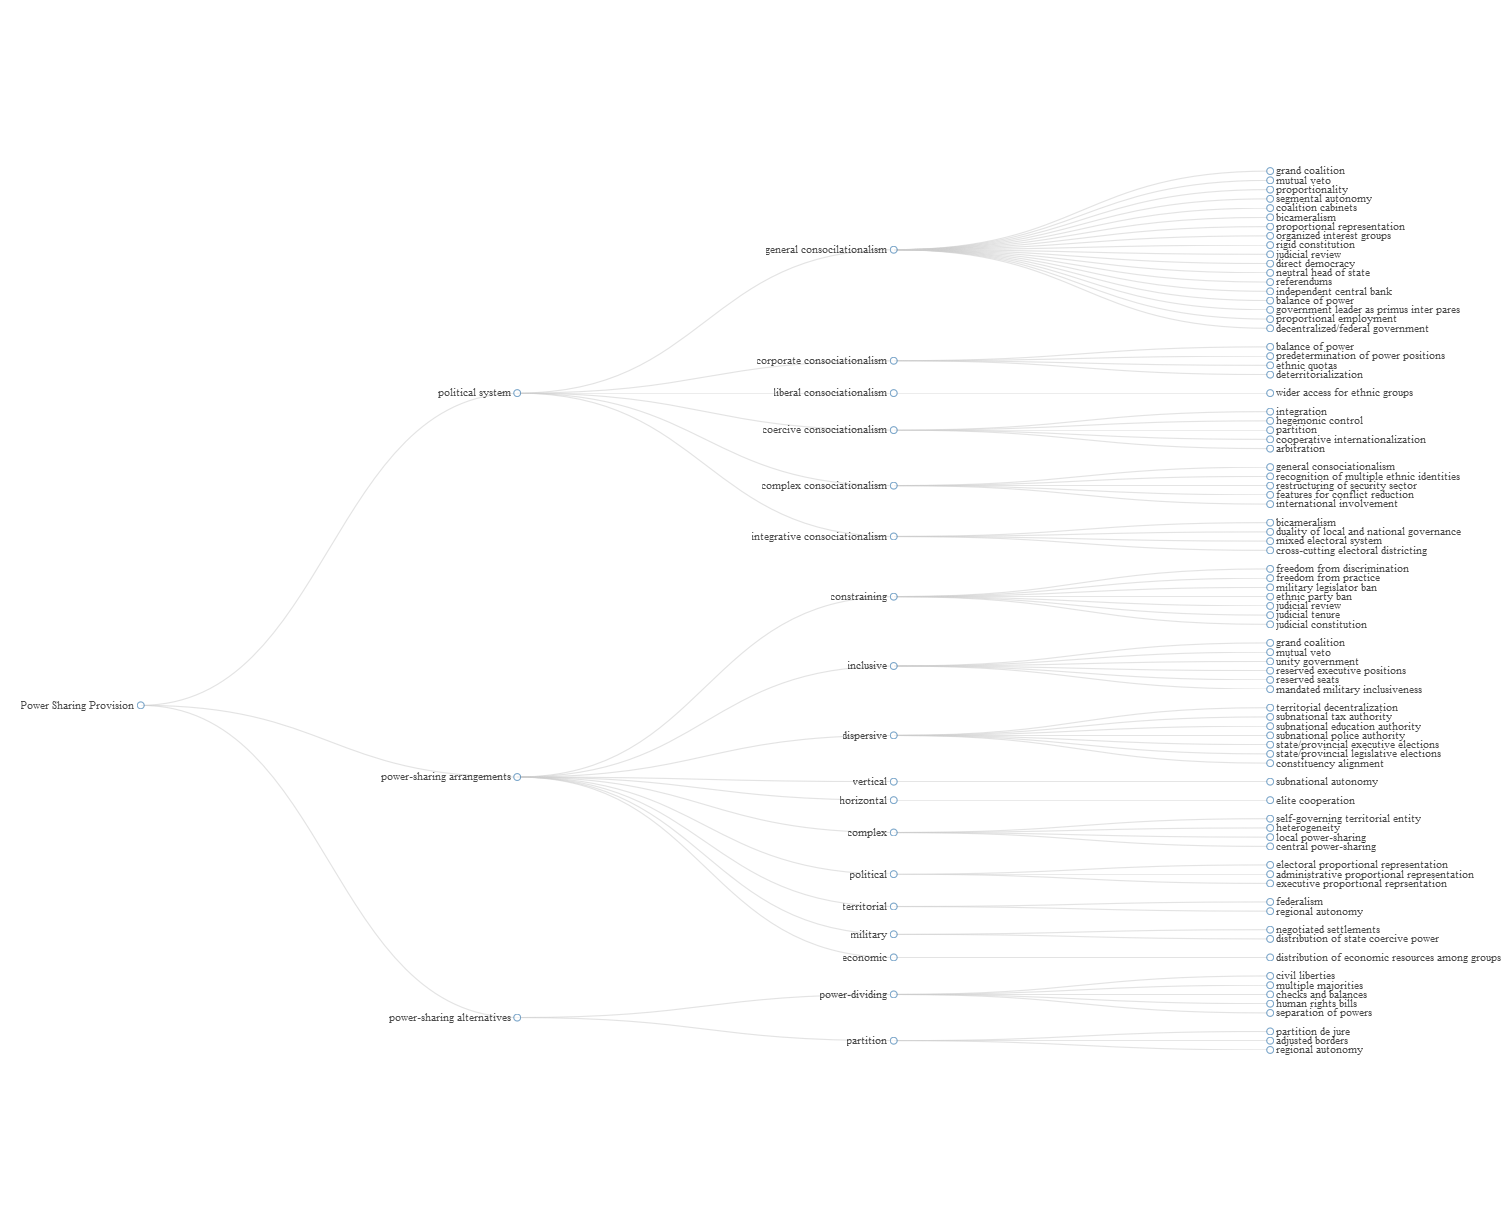
\includegraphics[width = 9.5in]{psp_ontology_vis.png}
	\caption{Full Ontology of Power-Sharing Provisions}
\end{sidewaysfigure}

\end{document}